\documentclass{article}
\usepackage{graphicx}

\begin{document}
\title{Project 5:  parallel primes}
\author{Robert L. Phillips III}
\maketitle
\newpage
\tableofcontents
\newpage

\section{Design}
\subsection{Files}
\begin{enumerate}
\item bitmask.c
\end{enumerate}

\subsection{bitmask.c}
\makebox[\textwidth]{\includegraphics[width=\textwidth]{flowchart.pdf}}

Because the program makes use of global variables, the different functionalities of the program were not separated out into different files like they have been in the past projects.\\\\

The Sieve of Eratosthenes is to be used in order to find the primes, so to begin, the array of unmarked bits will be split evenly between the number of desired threads/processes.  Each process will then mark all the multiples of the prime numbers in its given range as long as the multiple is less than the square root of the max value.  The main thread/parent process will then wait for all of the other threads/processes to finish before counting up the number of unmarked bits in the bitmap and printing the desired results to stdout.\\\\

The program will get the max value, the number of threads/processes, whether or not to print the primes and whether threads or processes should be used as command line parameters.  The threads/processes will all work on an array of unsigned chars as the bitmap.\\\\

For the parallel process case, the processes will work on a section of shared memory containing the bitmap.  The threaded case will use a global variable that all threads will be able to access and modify. No synchronization techniques should be necessary to implement this design.

\section{Work Log}
\begin{enumerate}
\item \textbf{Revision 1} (Wed 7 Nov 2012 10:33 AM) 1 hour:  Reworked the sieve algorithm so that it could work for the current project.  Optimized it for much quicker finding of primes.  Converted the prime finder to use a bitmap.
\item \textbf{Revision 2} (Thu 8 Nov 2012 9:09 AM) 2.2 hours:  Implemented the function to find the primes using threads.  Initial testing indicates some sort of race condition.
\item \textbf{Revision 3} (Mon 12 Nov 2012 10:00 AM) 1.5 hours:  Finalized the thread implementation.  No race condition was present.  The max value is not 4.3 billion, it is slightly less.
\item \textbf{Revision 4} (Wed 14 Nov 2012 12:21 PM) 1.4 hours:  Implemented the function to fork the processes and find the primes.  Moved the code to count and print the primes into their own functions.
\item \textbf{Revision 5} (Sat 17 Nov 2012 2:57 PM) 1 hour:  Wrote a script to run the prime finder enough times to generate the graphs and graphed the timings to a .ps file.
\item \textbf{Revision 6} (Sat 17 Nov 2012 5:40 PM) 3 hours:  Cleaned up the code for submission and finished the write up.
\end{enumerate}

\section{Timings}
\subsection{Graphs}
\makebox[\textwidth]{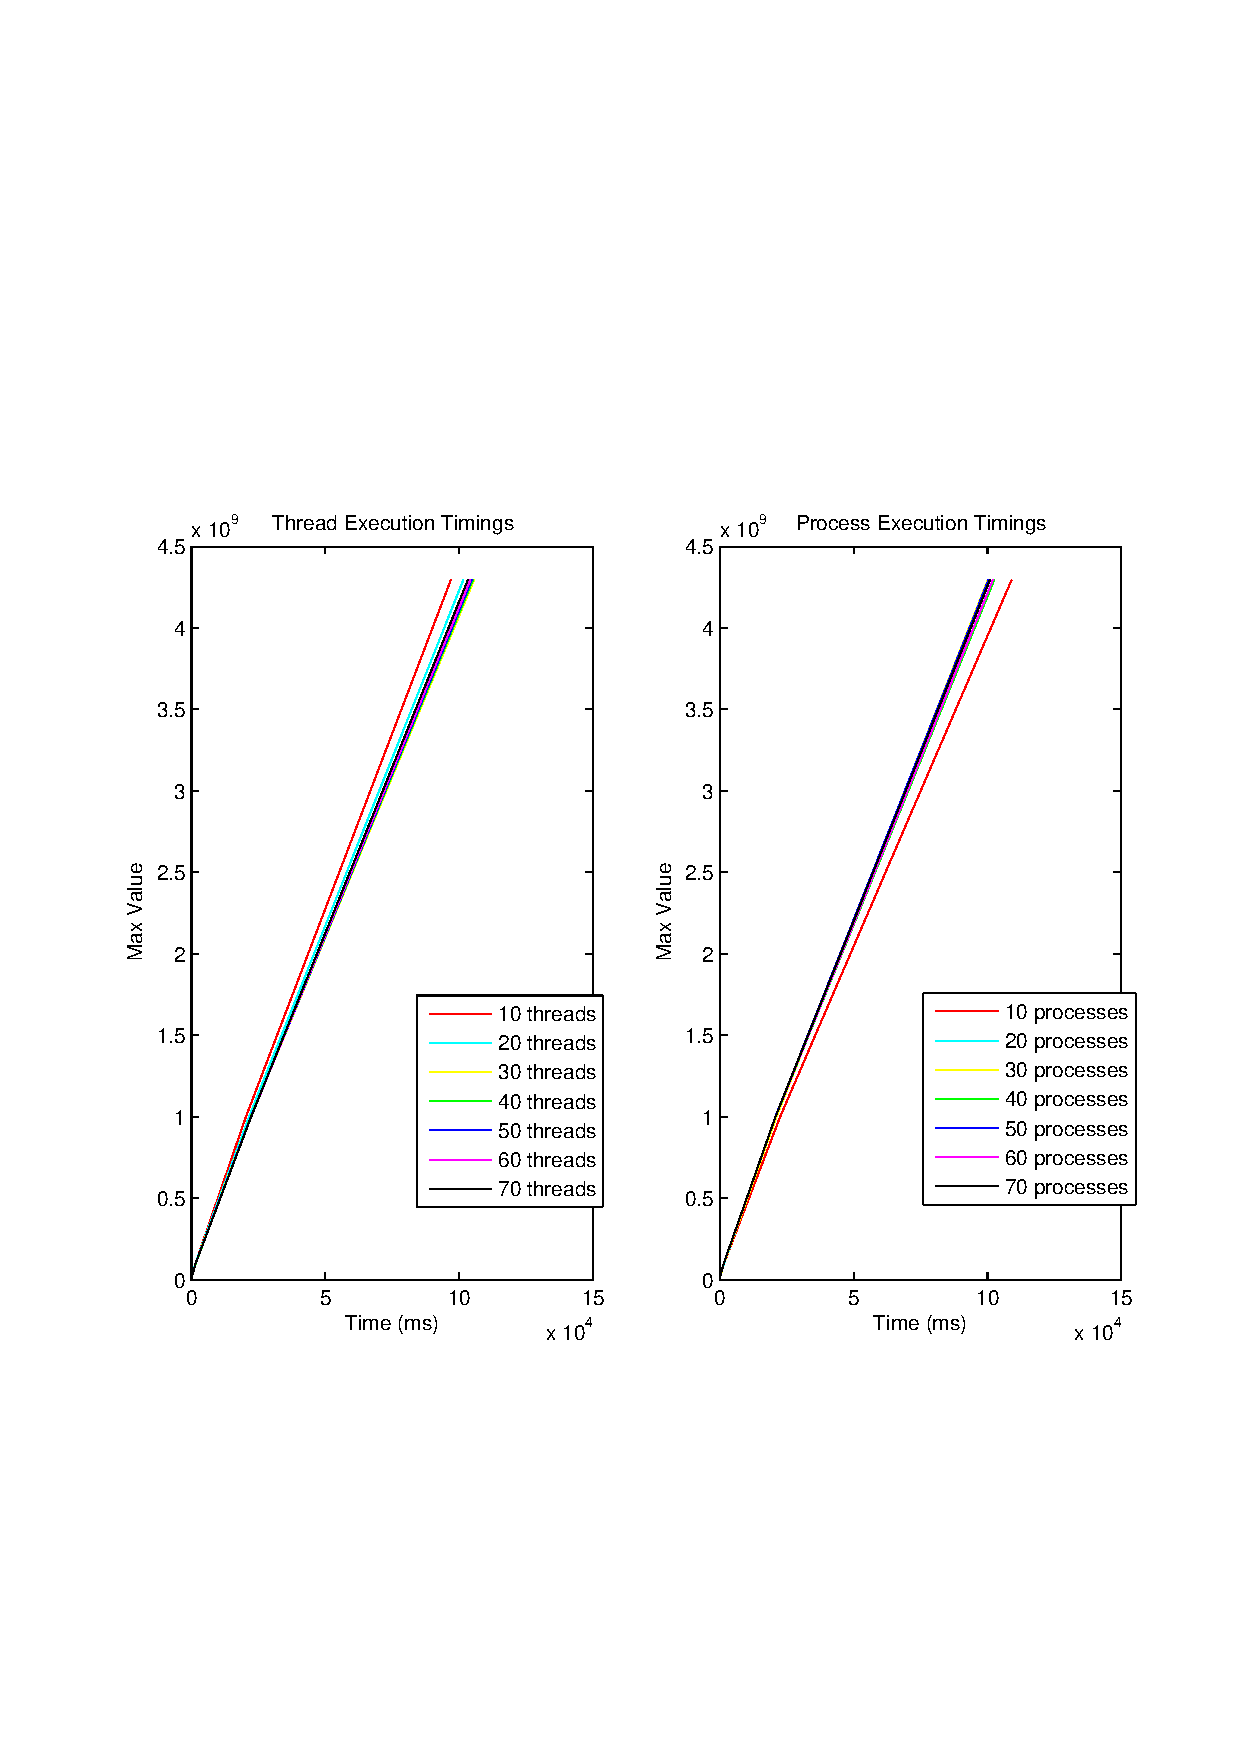
\includegraphics[width=\textwidth]{timing.pdf}}

\subsection{Program Output}
\begingroup
\obeylines
\input{time.txt}
\endgroup

\section{Additional Questions}
\begin{enumerate}
\item I believe the main point of this assignment is to get familiar with how to use the pthread functiosn and compare their use and performance to parallel programming using multiple processes.
\item In order to verify that my solution was correct, I simply ran the prime finder algorithm with different values for the number of threads/processes and different max values and verified that the output matched the output that I was expecting.
\item I learned what advantages and disadvantages there are to using threads vs. using processes.  I also learned how and why synchronization techniques need to be used in order to successfully compute different things in parallel and avoid race conditions.
\end{enumerate}


\end{document}
